% !TEX encoding = UTF-8
% !TEX TS-program = pdflatex
% !TEX root = ../tesi.tex

%**************************************************************
\chapter{Analisi dei requisiti}
\label{cap:analisi-requisiti}
%**************************************************************

\intro{Tale capitolo ha l’obiettivo di esporre e analizzare i requisiti espliciti e impliciti per la realizzazione del plugin Maven per la pubblicazione di documentazione software.
L'attività di analisi ha funto da base per la fase di progettazione del software, in modo che il prodotto fosse conforme alle richieste dell’azienda.}

% \section{Casi d'uso}

% Per lo studio dei casi di utilizzo del prodotto sono stati creati dei diagrammi.
% I diagrammi dei casi d'uso (in inglese \emph{Use Case Diagram}) sono diagrammi di tipo \gls{uml} dedicati alla descrizione delle funzioni o servizi offerti da un sistema, così come sono percepiti e utilizzati dagli attori che interagiscono col sistema stesso.
% Essendo il progetto finalizzato alla creazione di un tool per l'automazione di un processo, le interazioni da parte dell'utilizzatore devono essere ovviamente ridotte allo stretto necessario. Per questo motivo i diagrammi d'uso risultano semplici e in numero ridotto.

% \begin{figure}[!h]
%     \centering
%     \includegraphics[width=0.9\columnwidth]{usecase/scenario-principale}
%     \caption{Use Case - UC0: Scenario principale}
% \end{figure}

% \begin{usecase}{0}{Scenario principale}
% \usecaseactors{Sviluppatore applicativi}
% \usecasepre{Lo sviluppatore è entrato nel plug-in di simulazione all'interno dell'IDE}
% \usecasedesc{La finestra di simulazione mette a disposizione i comandi per configurare, registrare o eseguire un test}
% \usecasepost{Il sistema è pronto per permettere una nuova interazione}
% \label{uc:scenario-principale}
% \end{usecase}


% \begin{usecase}{1}{Configurazione}
% \usecaseactors{Sviluppatore}
% \usecasepre{Lo sviluppatore sta utilizzando il progetto}
% \usecasedesc{Lo sviluppatore configura come }
% \usecasepost{Il sistema è pronto per l'esecuzione}
% \label{uc:scenario-principale}
% \end{usecase}

\section{Premessa}
Il prodotto realizzato è un plugin Maven e possiede come nome ufficiale: \emph{Maven documentation publisher plug-in}.

L'obiettivo all'inizio dello stage era il semplice caricamento di documentazione archiviata su \emph{Docs} di Confluence, per questo motivo è stato scelto di creare il goal denominato \emph{publish}.
Successivamente, nel corso dello stage, sono state aggiunte delle nuove funzionalità e un nuovo goal, dato che le tempistiche pianificate erano ottimistiche e hanno permesso sufficiente tempo per ampliare il prodotto.


\section{Descrizione del prodotto}

\emph{Maven documentation publisher plug-in} supporta la pubblicazione di documentazione in formato HTML. Ha due goal:
\begin{itemize}
	\item \bd{publish}: che pubblica la documentazione;
	\item \bd{cleanup}: che elimina la documentazione contentente SNAPSHOT nel nome.
\end{itemize}
Il principale è \emph{publish} e si occupa della pubblicazione su  \emph{Docs} Confluence della documentazione del codice di un qualunque progetto Maven su cui è configurato il plugin.
Questo è possibile perché il plugin Docs di Confluence accetta archivi, ovvero file in formato .zip o .jar.
La documentazione in questo formato può essere per esempio la documentazione Javadoc (documentazione del codice sorgente scritto in linguaggio Java) o Open API (specifica per file di interfaccia leggibili dalle macchine per descrivere servizi web RESTful, conosciuta anche come specifica Swagger).
Entrambe Javadoc e Open API sono il tipo di documentazione di maggior interesse per l'azienda da pubblicare su Docs. \\
Ogni archivio caricato contribuisce alla creazione di una pagina \emph{doc}.
Ogni \emph{doc} viene identificato univocamente all'interno di una categoria, per questo motivo, il titolo deve essere unico.
Una pagina viene creata se il titolo della documentazione è nuovo, altrimenti la pagina già esistente viene semplicemente aggiornata. \\ 
 
\subsection{Il goal \emph{publish}} \label{goalPublish}
\emph{Maven documentation publisher plug-in} è altamente configurabile, in modo da soddisfare qualunque esigenza dello sviluppatore.
Innanzitutto esso consente all'utente di inserire:
\begin{itemize}
	\item la documentazione;
	\item le proprie credenziali per accedere a Confluence;	
	\item il nome della categoria in cui allocare la documentazione.
\end{itemize}
La documentazione che fornisce l'utente può essere di tre tipi:
\begin{enumerate}
	\item archivio (.zip o .jar);
	\item cartella (contentente più file HTML);
	\item singolo file HTML.
\end{enumerate}
Nei casi 2. e 3. il plugin si occupa anche dell'archiviazione. \\
I possibili modi per fornire le credenziali sono molteplici:
\begin{itemize}
	\item username e password vengono date direttamente nei campi della configurazione a loro destinati;
	\item username e password vengono prese dalla sezione server del file ``.m2/settings.xml'' in cui sono salvate criptate. \footnote{A questo scopo, l'utente deve aver prima proceduto con la criptazione delle proprie credenziali come spiegato alla pagina \url{https://maven.apache.org/guides/mini/guide-encryption.html}} 
\end{itemize}
Non è necessario che l'utente provveda entrambi i modi, ma almeno uno deve esserci.
Se ci sono entrambi, il plugin utilizza il prelevamento dal file ``settings.xml''. \\

Il sistema richiede obbligatoriamente dall'utente le infomazioni sopra descritte.
Oltre a ciò, esso prevede una configurazione di default.
Ognuno di questi parametri può essere facoltativamente cambiato dall'utente. 

	\subsubsection{Parametri opzionali} \label{parametriOpzionali}
	L'utente può scegliere nome e versione della documentazione.
	Il titolo della pagina \emph{doc} viene costruito dall'unione di nome e versione (ad esempio dato nome ``Docs Maven Plugin'' e versione ``2019'', il titolo apparirà come: ``Docs Maven Plugin 2019'').

	% TODO da posizionare
	% -------------------------

	Nel caso in cui l'utente non fornisca nome o versione, o nessuno dei due, il sistema prevede il seguente comportamento per i due parametri:
	\begin{itemize}
		\item \bd{nome}: preso dal nome del progetto o alternativamente dall'\emph{artifactId};
		\item \bd{versione}: preso dalla versione del progetto.
	\end{itemize} 

	Vengono riportati qui di seguito alcuni esempi:
	\begin{enumerate}
		\item nome documentazione = Quickstart Doc, versione documentazione = 2019, nome progetto = Quickstart Vogella project, versione progetto = 2.1.1-SNAPSHOT, artifactId = quickstart
		\item nome progetto = Quickstart Vogella project, versione progetto = 2.1.1-SNAPSHOT,  artifactId= quickstart
		\item versione documentazione = 2018, versione progetto = 2.1.1-SNAPSHOT,  artifactId= quickstart
	\end{enumerate}

	\begin{figure}[H]
		\centering
		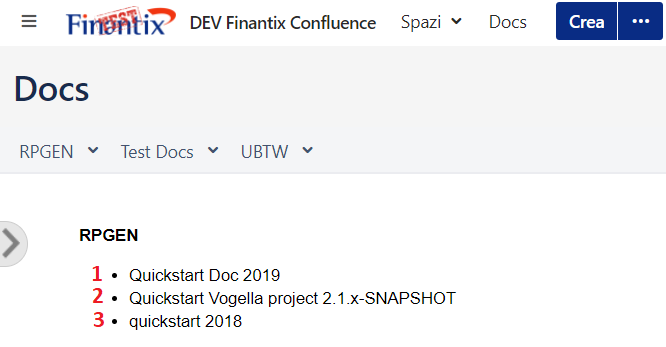
\includegraphics[width=0.85\textwidth]{immagini/DocsExamples.png}\\
		\caption{Screenshot di esempi di titoli di pagine doc}
		\label{screenDocsNameVersion}
	\end{figure}

	Come è possibile vedere dall'immagine \ref{screenDocsNameVersion}, nel caso 1. vengono dati dall'utente sia nome che versione della documentazione, per questo il titolo viene costruito con questi valori.
	Nel caso 2. invece non viene fornito nessuno dei due e per questo viene utilizzato il nome e la versione del progetto. 
	Nel caso 3. viene data solo la versione della documentazione, che infatti viene preferita alla versione del progetto, ma non il nome della documentazione. 
	Poichè nemmeno il nome del progetto è configurato nel POM del progetto, viene scelto di utlizzare l'ultima opzione rimanente: l'artifactId.

	% ---------------------------

	L'utente può inoltre decidere di impostare:
	\begin{itemize}
		\item lo skip (salto) dell'esecuzione del plugin;
		\item che il plugin non fallisca nel caso in cui accada qualche errore del client;
		\item i tipi di progetto supportati dal plugin;
		\item i tipi di progetto a cui il plugin non deve dare dei warning (messaggi di avvertimento);
		\item che il plugin non fallisca nel caso in cui il percorso all'archivio dato dall'utente come documentazione da caricare non esista.
	\end{itemize}

	Per di più, nel caso in cui la documentazione non sia di tipo archivio, bensì il percorso ad una cartella, è possibile dare delle ulteriori istruzioni:
	\begin{itemize}
		\item dove salvare l'archivio creato;
		\item quali tipi di file includere nell'archivio;
		\item quali tipi di file escludere dall'archivio.
	\end{itemize}

	Ogni archivio caricato su \emph{Docs} plugin di Confluence deve contenere al suo interno una pagina denominata \emph{main entrance page}, la quale essenzialmente è la prima pagina che viene visualizzata quando si entra nella pagina \emph{doc}.
	Questa è impostata di default nel plugin come ``index.html''.
	Per questo motivo è stato scelto di permettere a \emph{Maven documentation publisher plug-in} di creare questo file qualora mancasse.
	Esso indirizza automaticamente ad un altro file della documentazione: un file principale che scelto dall'utente tramite l'inserimento del nome in fase di configurazione.


\subsection{Il goal \emph{cleanup}}
Il secondo \emph{goal}, \emph{cleanup}, è nato dalla necessità di eliminare la documentazione relativa ad un prodotto che non è stato rilasciato.
Questo tipo di prodotti presentano ``SNAPSHOT'' nella versione e per questo motivo, anche il titolo della pagina \emph{doc} lo contiene.
Si ha quindi qui a che vedere con la pulizia totale dal plugin \emph{Docs} di tutte queste pagine. \\
A questo scopo non è necessario aggiungere nulla alla configurazione del plugin: sono sufficienti le credenziali dell'utente. 

% Main goal is publish and it is bound to package life cycle phase. 

% Furthermore a doc page can be overall identified by its docKey, which is a sequence of category id and doc id.


\newpage

\section{Requisiti}
Ad ogni requisito viene assegnato il codice identificativo univoco:
	\begin{center}
		\texttt{R[Numero][Tipo][Priorità]}
	\end{center}
	in cui ogni parte ha un significato preciso:
	\begin{itemize}
		\item \textbf{R}: requisito.
		\item \textbf{Numero}: numero progressivo che segue una struttura gerarchica.
		\item \textbf{Tipo}: la la tipologia di requisito che può essere di:
		\begin{itemize}
			\item \textbf{F}: funzionalità.
			\item \textbf{Q}: qualità.
			\item \textbf{V}: vincolo.
		\end{itemize}
		\item \textbf{Priorità}: indica il grado di urgenza di un requisito di essere soddisfatto, come:
		\begin{itemize}
			\item \textbf{0}: opzionale.
			\item \textbf{1}: desiderabile.
			\item \textbf{2}: obbligatorio.
		\end{itemize}
	\end{itemize}


	Esempio: \texttt{R2Q1} indica il secondo requisito di qualità ed è desiderabile. \\

	I requisiti individuati sono riassunti in tabelle secondo la loro tipologia.
	Inoltre, tutti i requisiti individuati e scelti dalla candidata, presentano nella tabella come fonte ``Interno'' e come grado di urgenza ``0'' poichè il loro soddisfacimento non è strettamente necessario.


% Da un'attenta analisi dei requisiti e dei casi d'uso effettuata sul progetto, è stata stilata la tabella che traccia tutti i requisiti in rapporto alle loro fonti.

% \newpage

	% TODO dividere i requisiti in altri gruppi e dare una spiegazione
	\subsection{Requisiti di funzionalità}\label{RequisitiFunzionalità}
	I requisiti di funzionalità sono ulteriormenti suddivisi in tabelle secondo:
	\begin{itemize}
		\item requisiti relativi a ciò che il sistema permette all'utente di configurare;
		\item requisiti relativi a messaggi di errore che il sistema deve essere in grado di lanciare;
		\item requisiti relativi a generiche funzionalità del sistema.
	\end{itemize}
	Per ogni tabella, i primi requisiti, segnalati come obbligtori, sono i requisiti identificati all'inizio del progetto, essenziali per il funzionamento del plugin.
	I requisiti elencati successivamente come desiderabili sono invece le funzionalità aggiunte in un secondo momento, nel corso dello stage, come quanto accennato nella premessa all'inizio di questo capitolo.
	All'interno della descrizione del requisito si utilizzano alcune abbreviazioni per semplificare la lettura della tabella:
	\begin{itemize}
		\item ``Inserimento'' per ``L'utente nella configurazione deve poter inserire'';
		\item ``Errore se'' per ``Il sistema deve dare un messaggio di errore qualora''.
	\end{itemize}
		 

	% \stepcounter{tableCounter}
	\begin{table}[H]
		\begin{paddedtablex}[1.7]{\textwidth}{cXc}%0 opz  2 obb
			\rowcolor{beautyblue} \textbf{Codice} & \textbf{Descrizione} & \textbf{Fonte} \\\toprule
			
			\ReqF{2}{Inserimento documentazione}{Azienda}
				\subReqF{2}{Inserimento archivio (.zip o .jar)}{Azienda}
				\subReqF{1}{Inserimento file html}{Azienda}
				\subReqF{1}{Inserimento cartella}{Azienda}	
            \ReqF{2}{Inserimento credenziali}{Azienda}
			    \subReqF{2}{Inserimento username}{Azienda}
				\subReqF{2}{Inserimento password}{Azienda}
				\subReqF{2}{Inserimento identificativo server}{Azienda}
			\ReqF{2}{Inserimento nome della categoria Confluence in cui allocare la documentazione}{Azienda}	
			\ReqF{2}{Inserimento nome della documentazione}{Azienda}
			\ReqF{2}{Inserimento versione della documentazione}{Azienda}
			\ReqF{2}{L'utente deve poter configurare il plugin in modo che esso ne salti la propria esecuzione}{Azienda}
			\ReqF{1}{Inserimento luogo in cui l'archivio viene salvato all'interno del progetto}{Azienda}
			\ReqF{1}{Inserimento tipologie di file attinenti alla documentazione}{Azienda}
				\ReqF{1}{Inserimento tipologie di file da includere nella cartella}{Azienda}
				\ReqF{1}{Inserimento tipologie di file da escludere dalla cartella}{Azienda}
			\ReqF{1}{Inserimento nome del file principale della documentazione}{Azienda}
			\ReqF{1}{L'utente deve poter configurare il plugin in modo che esso non fallisca se avvengono errori del client}{Azienda}
			\ReqF{1}{Inserimento tipi di progetto supportati dal plugin}{Azienda}
			\ReqF{1}{Inserimento tipi di progetto a cui il plugin non deve dare messaggi di warning}{Azienda}
			\ReqF{1}{L'utente deve poter configurare il plugin in modo che esso non fallisca se l'archivio dato non esiste}{Azienda}
			
			\bottomrule
		\end{paddedtablex}
		\caption{Elenco dei requisiti di funzionalità}
	\end{table}


	\begin{table}[H]
		\begin{paddedtablex}[1.7]{\textwidth}{cXc}%0 opz  2 obb
			\rowcolor{beautyblue} \textbf{Codice} & \textbf{Descrizione} & \textbf{Fonte} \\\toprule
			
			\ReqF{2}{Errore se l'utente non fornisce nessuna documentazione}{Azienda}
			\ReqF{2}{Errore se l'archivio dato non esiste}{Azienda}	
			\ReqF{2}{Errore se l'utente non fornisce le proprie credenziali}{Azienda}
			\ReqF{2}{Errore se la categoria non è stata aggiunta}{Azienda}
			\ReqF{1}{Errore se il file indicato dall'utente come file principale della cartella non esiste}{Azienda}

			\bottomrule
		\end{paddedtablex}
		\caption{Elenco dei requisiti di funzionalità relativi ai messaggi di errore
		% (\thetableCounter)
		}
	\end{table}

	\begin{table}[H]
		\begin{paddedtablex}[1.7]{\textwidth}{cXc}%0 opz  2 obb
			\rowcolor{beautyblue} \textbf{Codice} & \textbf{Descrizione} & \textbf{Fonte} \\\toprule

			\ReqF{2}{Il sistema deve fornire delle proprietà per tutti gli elementi configurabili dall'utente}{Azienda}
			\ReqF{2}{Il sistema deve essere in grado di costruire il titolo della pagina contenente la documentazione, a partire da nome e versione della documentazione}{Azienda}
			\ReqF{1}{Il sistema deve permettere lo skip dell'esecuzione del plugin, nel caso in cui il progetto compilato non sia tra i tipi supportati}{Azienda}
			\ReqF{1}{L'utente deve poter eliminare tutta la documentazione con versione ``SNAPSHOT'' presente}{Azienda}

			\bottomrule
		\end{paddedtablex}
		\caption{Elenco dei requisiti di funzionalità del sistema
		% (\thetableCounter)
		}
	\end{table}



	% \setcounter{tableCounter}{1}
	% NB: molti requisiti di qualità sono stati tolti perchè non sono veri requisiti del sistema, riguardano noi e il nostro modo di fare, non il sistema
	\subsection{Requisiti di qualità}\label{RequisitiQualita}


	\begin{table}[H]
		\begin{paddedtablex}[1.7]{\textwidth}{cXc}
			\rowcolor{beautyblue}\textbf{Codice} & \textbf{Descrizione} & \textbf{Fonte} \\
			\toprule
			
			\ReqQ{2}{Le norme presenti sulla wiki aziendale devono essere rispettate}{Azienda}
				% \subReqQ{1}{Ogni commit effettuato deve rispettare la formattazione descritta nella wiki}{Azienda}
				\subReqQ{2}{Il nome di ogni variabile, classe, ecc nel codice deve essere significativo}{Azienda}
				\subReqQ{2}{I commenti nel codice devono essere facilmente comprensibili}{Azienda}
				\subReqQ{2}{Il codice non deve contenere violazioni di SonarQube con alta severità}{Azienda}
				\subReqQ{2}{La copertura dei test deve essere almeno pari al 70\% del codice}{Azienda}

			\bottomrule
		\end{paddedtablex}
		\caption{Elenco dei requisiti di qualità (1)}
	\end{table}


	\begin{table}[H]
		\begin{paddedtablex}[1.7]{\textwidth}{cXc}
			\rowcolor{beautyblue}\textbf{Codice} & \textbf{Descrizione} & \textbf{Fonte} \\
			\toprule

			\ReqQ{2}{Devono essere forniti test realizzati con JUnit che verifichino la copertura di tutti i parametri disponibili nella configurazione}{Azienda}
			\ReqQ{2}{Deve essere redatto un manuale utente}{Azienda}
				\subReqQ{2}{Deve essere redatta una pagina Confluence che descriva come configurare il plugin}{Azienda}
				\subReqQ{1}{Deve essere redatta una pagina di utilizzo Maven ``Usage'' che descriva tutti i possibili utilizzi del plugin}{Azienda}
			\ReqQ{2}{Deve essere redatto un manuale dello sviluppatore}{Azienda}
				\subReqQ{2}{Deve essere redatta una pagina Confluence che descriva la progettazione del plugin tramite diagrammi}{Azienda}
				\subReqQ{2}{Deve essere redatta e generata la documentazione Javadoc del plugin}{Azienda}
			\ReqQ{0}{Il nome di ogni test realizzato con JUnit deve iniziare con ``test''}{Interno}
			\ReqQ{0}{Il nome di ogni test realizzato con JUnit deve rispettare la notazione camel case}{Interno}
			\ReqQ{0}{Ogni messaggio di errore del plugin deve essere sufficientemente esplicativo}{Interno}

			\bottomrule
		\end{paddedtablex}
		\caption{Elenco dei requisiti di qualità (2)}
	\end{table}



	\subsection{Requisiti di vincolo}\label{RequisitiVincolo}

	\begin{table}[H]
		\begin{paddedtablex}[1.7]{\textwidth}{cXc}
			\rowcolor{beautyblue}\textbf{Codice} & \textbf{Descrizione} & \textbf{Fonte} \\
			\toprule

			\ReqV{2}{Il plugin deve essere sviluppato nel linguaggio di programmazione Java}{Azienda}
			\ReqV{2}{Il plugin deve essere testato tramite JUnit}{Azienda}
			\ReqV{2}{Come ambiente di sviluppo è necessario utilizzare Eclipse}{Azienda}
			\ReqV{2}{Per la build dei progetti è necessario utilizzare Maven}{Azienda}
			\ReqV{2}{Per la pubblicazione di documentazione è necessario utilizzare Confluence}{Azienda}


			\bottomrule
		\end{paddedtablex}
		\caption{Elenco dei requisiti di vincolo (1)}
	\end{table}


	\begin{table}[H]
		% \centering
		% {\def\arraystretch{1.7}
		% \begin{tabularx}{\textwidth}{cXc}
		\begin{paddedtablex}[1.7]{\textwidth}{cXc}
			\rowcolor{beautyblue}\textbf{Codice} & \textbf{Descrizione} & \textbf{Fonte} \\
			\toprule

			\ReqV{2}{I requisiti identificati devono essere tracciati su Jira}{Azienda}
			\subReqV{2}{Lo stato di ogni requisito presente su Jira deve sempre essere opportunamente aggiornato}{Azienda}
			\ReqV{2}{Come strumento di Continuous integration è necessario utilizzare Jenkins}{Azienda}
			\ReqV{2}{Per l'analisi statica del codice è necessario utilizzare SonarQube}{Azienda}
			\ReqV{2}{Per il controllo di versione del codice è necessario utilizzare Bitbucket}{Azienda}
			\ReqV{2}{Utilizzare JUnit per realizzare test di unità}{Azienda}
			\ReqV{0}{Utilizzare GitKraken come client di Git}{Interno}
			\ReqV{0}{Utilizzare Visual Studio Code come editor per il codice}{Interno}
			\ReqV{0}{Utilizzare SequenceDiagram.org per la creazione dei diagrammi di sequenza}{Interno}
			\ReqV{0}{Utilizzare ObjectAid UML Explorer per la creazione dei diagrammi delle classi}{Interno}
			\ReqV{0}{Utilizzare Meecrowave per la creazione di un semplice server}{Interno}

			\bottomrule
		\end{paddedtablex}
		\caption{Elenco dei requisiti di vincolo (2)}
	\end{table}


	\subsection{Riepilogo dei requisiti}

	\begin{table}[H]
		\centering
		{\def\arraystretch{1.7}
		\begin{tabularx}{\textwidth}{XXXX}
			\rowcolor{beautyblue} \textbf{Tipologia} & \textbf{Obbligatori} & \textbf{Desiderabili} & \textbf{Opzionali} \\\toprule
			Di funzionalità & 16 & 14 & 0 \\
			Di qualità & 11 & 1 & 3 \\
			Di vincolo & 11 & 0 & 5
			\\\bottomrule
		\end{tabularx}}
		\caption{Riepilogo dei requisiti}
	\end{table}





% \begin{table}%
% \caption{Tabella del tracciamento dei requisiti di vincolo}
% \label{tab:requisiti-vincolo}
% \begin{tabularx}{\textwidth}{lXl}
% \hline\hline
% \textbf{Requisito} & \textbf{Descrizione} & \textbf{Use Case}\\
% \hline
% RVO-1    & La libreria per l'esecuzione dei test automatici deve essere riutilizzabile & - \\
% \hline
% \end{tabularx}
% \end{table}%